\documentclass[11pt,a4paper]{moderncv}
\moderncvtheme[blue]{banking}                
\usepackage[utf8]{inputenc}
\usepackage[top=0.9cm, bottom=0.9cm, left=1.4cm, right=1.4cm]{geometry}
\usepackage[english]{babel}
\setlength{\hintscolumnwidth}{2.9cm} % width of the left column (dates)
%\setlength{\makecvtitlenamewidth}{20cm}
%\setlength{\maketitlewidth}{\textwidth}
%\setlength{\maketitleboxwidth}{\textwidth}
%\setlength{\maketitlewidth}{\textwidth}
%\setlength{\quotewidth}{0.9\textwidth}

\firstname{Romain}
\familyname{Pellerin}
\title{Software developer}
%\photo[64pt][0.0pt]{picture} % '64pt' is the height the picture must be resized to, 0.0pt is the thickness of the frame around it (put it to 0pt for no frame) and 'picture' is the name of the picture file       
\address{9 rue des réservoirs}{60200 Compiègne}{France}  
\email{contact@romainpellerin.eu}                      
\homepage{romainpellerin.eu}
\mobile{+33-7 85 25 71 64} 
%\extrainfo{21 years old -- Driving licence}
\quote{Objective: a 6-month internship in software development starting from September 2015}
\renewcommand*{\quotefont}{\Large\bfseries}

% I took the original code from moderncvstylebanking.sty and changed line 28
\makeatletter
\renewcommand*{\maketitle}{%
  \setlength{\maketitlewidth}{1.0\textwidth}%
  \hfil%
  \parbox{\maketitlewidth}{%
    \centering%
    % name and title
    \namestyle{\@firstname~\@lastname}%
    \ifthenelse{\equal{\@title}{}}{}{\titlestyle{~|~\@title}}\\% \isundefined doesn't work on \@title, as LaTeX itself defines \@title (before it possibly gets redefined by \title) 
    % detailed information
    \addressfont\color{color2}%
    \ifthenelse{\isundefined{\@addressstreet}}{}{\addtomaketitle{\addresssymbol\@addressstreet}%
      \ifthenelse{\equal{\@addresscity}{}}{}{\addtomaketitle[~--~]{\@addresscity}}% if \addresstreet is defined, \addresscity and \addresscountry will always be defined but could be empty
      \ifthenelse{\equal{\@addresscountry}{}}{}{\addtomaketitle[~--~]{\@addresscountry}}%
      \flushmaketitle\@firstmaketitleelementtrue\\}%
    \collectionloop{phones}{% the key holds the phone type (=symbol command prefix), the item holds the number
      \addtomaketitle{\csname\collectionloopkey phonesymbol\endcsname\collectionloopitem}}%
    \ifthenelse{\isundefined{\@email}}{}{\addtomaketitle{\emailsymbol\emaillink{\@email}}}%
    \ifthenelse{\isundefined{\@homepage}}{}{\addtomaketitle{\homepagesymbol\httplink{\@homepage}}}%
    \collectionloop{socials}{% the key holds the social type (=symbol command prefix), the item holds the link
      \addtomaketitle{\csname\collectionloopkey socialsymbol\endcsname\collectionloopitem}}%
    \ifthenelse{\isundefined{\@extrainfo}}{}{\addtomaketitle{\@extrainfo}}%
    \flushmaketitle}\\[2.5em]}% need to force a \par after this to avoid weird spacing bug at the first section if no blank line is left after \maketitle
 \makeatother

\begin{document}
\makecvtitle

\section{Professional Experience}
\cventry{September 2014 -- present}{Computer Science Project Manager}{\href{http://www.usec-utc.fr/}{USEC}}{Compiègne (France)}{}{I am in charge of software development projects. I help our clients throughout the process, ensuring total satisfaction from specifying their needs to implementation and testing. The tech part of each project is made by students (developers).
\begin{itemize}
  \item Writing official documents (quotes, specifications, customer agreements, etc.)
  \item Recruiting and mentoring students (first of developers, and since January of other CS project managers)
\end{itemize}}
\cventry{June 2013 -- September 2014}{Android and web developer}{Self-employed (\textit{Auto-entrepreneur})}{Nantes (France)}{}{Developed and updated the Android application and the website of the startup \textsc{\href{http://www.who-wanna.com/en/}{WhoWanna}}.}%\newline{}

\cventry{April 2014 -- June 2014}{Intern in software development}{\href{http://www.who-wanna.com/en/}{WhoWanna}}{Nantes (France)}{}{
\begin{itemize}%
\item Migrated data onto a "cloud" solution (\href{http://www.clever-cloud.com/}{Clever Cloud})
\item Updated the Android application (added some features, graphical update)
\item Started a change in the language and the DBMS used on the server: from PHP to Scala and from MySQL to PostgreSQL
\item Wrote internal documentation (\LaTeX{} and a website) and set up a versioning system (Git)
\end{itemize}}

\cventry{October 2013 -- March 2014}{Member of a college project}{\href{http://www.iutnantes.univ-nantes.fr/321/0/fiche___formation/}{Nantes University Institute of Technology (IUT de Nantes)}}{Nantes (France)}{}{Coordinated the development of a streaming server on a Raspberry-Pi (group project). I carried out the server development (Tomcat/Java EE) and the Android application development (Java).}

\section{Education}
\cventry{2014 -- present}{First year engineering student (Première année du cycle ingénieur)}{\href{http://www.utc.fr/formations-enseignements/genie-informatique.php}{Université de Technologie de Compiègne}}{Compiègne (France)}{}{Majoring in Computer Science} % year, degree, institution, city+picture = {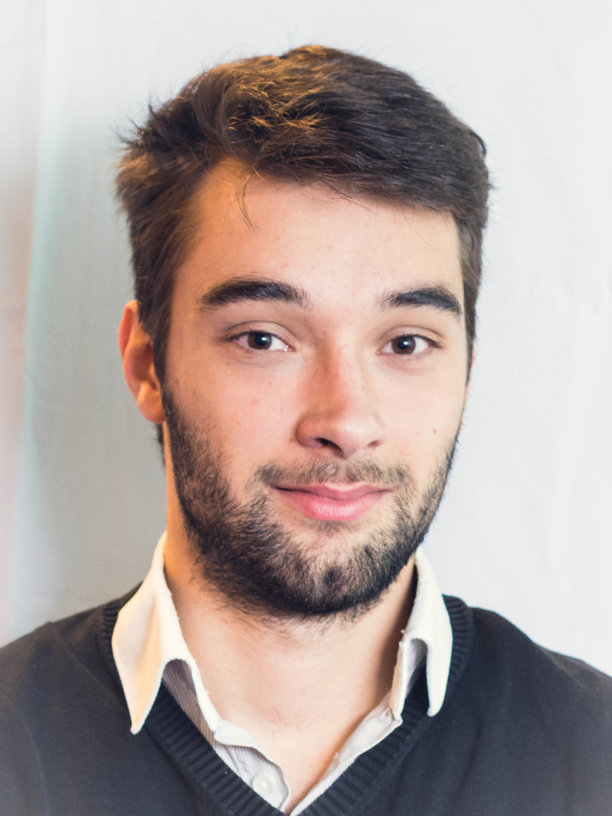
\includegraphics[scale=0.5]{picture}City}, grade, description
\cventry{2012 -- 2014}{Two-year core studies diploma in Computer Science (DUT Informatique)}{\href{http://www.iutnantes.univ-nantes.fr/321/0/fiche___formation/}{Nantes University Institute of Technology (IUT de Nantes)}}{Nantes (France)}{}{}

\section{Computer skills}
% \cvcomputer{category}{programs}{category}{programs}
% \cvdoubleitem{subtitle}{text}{subtitle}{text}
\cvitem{Programming languages}{C, C++, Java (SE \& EE), PHP, HTML, CSS, JavaScript, Bash, x86 assembly}
\cvitem{Modeling}{UML}
\cvitem{Databases}{Oracle, MySQL, PostgreSQL, Microsoft SQL Server (notions)}
\cvitem{Operating systems}{GNU/Linux (Debian), Windows XP/7/8}
\cvitem{Other}{Apache2, iptables, fail2ban, OpenVPN, Git, Subversion, TCP/IP}
%\cvitem{Software}{LaTeX, Microsoft Office, LibreOffice, Adobe Photoshop}

\section{Languages and other skills}
\cvlanguage{French}{Mother tongue}{}
\cvlanguage{English}{European B2 level (Independent User: Upper intermediate)}{\textbf{Toeic 895/990}}
\cvitem{Other}{Knowledge in communication and business management (courses of DUT Informatique)}

\section{Hobbies}
\cvdoubleitem{Computer Science meetings}{\href{http://devfest.gdgnantes.com/}{DevFest} (Nantes, France), \href{http://web2day.co/}{Web2Day} (Nantes, France)}{Free software}{Fervent defender, I often push code on \href{https://github.com/rpellerin}{GitHub}}
\cvdoubleitem{Music}{I have been playing the guitar for nine years}{Sport}{Workout, badminton}
\cvdoubleitem{Raspberry Pi}{Self-hosted websites, VPN, ownCloud}{}{}
\end{document}
